
%% bare_conf.tex
%% V1.3
%% 2007/01/11
%% by Michael Shell
%% See:
%% http://www.michaelshell.org/
%% for current contact information.
%%
%% This is a skeleton file demonstrating the use of IEEEtran.cls
%% (requires IEEEtran.cls version 1.7 or later) with an IEEE conference paper.
%%
%% Support sites:
%% http://www.michaelshell.org/tex/ieeetran/
%% http://www.ctan.org/tex-archive/macros/latex/contrib/IEEEtran/
%% and
%% http://www.ieee.org/

%%*************************************************************************


\documentclass[conference]{IEEEtran}


% *** CITATION PACKAGES ***


% *** GRAPHICS RELATED PACKAGES ***
\usepackage[mediumspace,mediumqspace,Gray,squaren,binary]{SIunits}
\usepackage{array}
\usepackage{graphicx,subfigure}

\newcommand{\subscript}[1]{\ensuremath{_{\textrm{#1}}}}


\begin{document}
%
% paper title
% can use linebreaks \\ within to get better formatting as desired
\title{A Software Defined Radio Gateway for \\
Wireless Sensor Networks}


% author names and affiliations
% use a multiple column layout for up to three different
% affiliations
% \author{
% \IEEEauthorblockN{Roberto de Matos and\\ 
%                   Leandro Buss Becker}
% \IEEEauthorblockA{Department of Automation and Systems\\
%                   Federal University of Santa Catarina (UFSC)\\
%                   Florian\'{o}polis - Brazil\\
%                   Email: \{rmatos,lbecker\}@das.ufsc.br}
% \and
% \IEEEauthorblockN{Tiago Rog\'{e}rio M\"{u}ck and \\
%                   Ant\^{o}nio Augusto Fr\"{o}hlich}
% \IEEEauthorblockA{Laboratory for Software and Hardware Integration\\
%                   Federal University of Santa Catarina (UFSC)\\
%                   Florian\'{o}polis - Brazil\\
%                   Email: \{tiago,guto\}@lisha.ufsc.br}
% }


% for over three affiliations, or if they all won't fit within the width
% of the page, use this alternative format:
% 
\author{\IEEEauthorblockN{Roberto de Matos\IEEEauthorrefmark{1},
Tiago Rog\'{e}rio M\"{u}ck\IEEEauthorrefmark{2},
Ant\^{o}nio Augusto Fr\"{o}hlich\IEEEauthorrefmark{2} and
Leandro Buss Becker\IEEEauthorrefmark{1}}
\IEEEauthorblockA{Federal University of Santa Catarina (UFSC)\\
                  Florian\'{o}polis - Brazil}
\IEEEauthorblockA{\IEEEauthorrefmark{1}Department of Automation and Systems (DAS)\\
                  Email: \{rmatos,lbecker\}@das.ufsc.br}
\IEEEauthorblockA{\IEEEauthorrefmark{2}Laboratory for Software and Hardware Integration (LISHA)\\
Email: \{tiago,guto\}@lisha.ufsc.br}}



% use for special paper notices
%\IEEEspecialpapernotice{(Invited Paper)}


% make the title area
\maketitle


\begin{abstract}
%\boldmath
The fast proliferation of Wireless Sensors Networks has triggered new fields of research related to communication reliability, implying the need to ensure connectivity among heterogeneous WSNs and the outside world. Thereby it is possible to enhance the availability of the data being transmitted in these networks. Due to the very limited power and computational resources of WSN nodes, communication with other networks is typically made through external gateways. This paper proposes the use of Software Defined Radio (SDR) to allow changes in the physical layer of the gateways in order to increase the flexibility in WSN communications. To exemplify our proposal we developed a gateway for 802.15.4 and 802.11b wireless networks. This example is used to evaluate critical parameters in such scenario, such as the impact of latency caused by the physical layer reconfiguration. 
\end{abstract}


\section{Introduction}
The popularization of Wireless Sensor Networks (WSN) has allowed the monitoring of many environments, such as home security, industrial fault diagnosis, chemical and biological detection or medical and environmental monitoring. The proliferation of these networks has triggered new field of research related to communication reliability, implying the need to ensure connectivity among heterogeneous WSNs and the outside world. Thereby it is possible to enhance the availability of the data being transmitted in these networks, as in many application scenarios this data should be made available in the outside world.

The very limited power and computational resources of WSN nodes require efficient operation and power management, which are not available in traditional communication radios and high overhead protocols, like IEEE 802.11 and TCP/IP~\cite{wu:2007,luo:2004}. Thus, proprietary protocols and low-power radios are used in WSNs, such as 802.15.4 and proprietary solutions, i.e. CC1000 (433MHz or 900MHz), which integrates Berkley's Mote Mica2. Therefore, it is necessary to use of gateways to interconnect WSNs themselves or connect WSNs and Area Networks (WAN, LAN or Cell phone networks)~\cite{hwang:2003,wu:2007}.

Research in WSN gateways has focused on aid and to allow flexibility to project with a bigger number of protocols.~\cite{wu:2007} provides a modular application layer WSN gateway framework that allows the gateway to be deployed in heterogeneous network environments and enables remote upgrading.~\cite{dunkels:2007} presents a communication architecture that adapts to a wide range of underlying communication mechanisms, from the MAC layer to the transport layer, without requiring any changes to applications or protocols.~\cite{hwang:2003} presents the architecture of the sensor gateway for web-based management. 

All these schemes allow a combination of some protocols requiring, or not, changes to the applications. However, the flexibility of these architectures can be used only on software layers of the communication protocols, so they are limited by the physical layers defined at project time. This paper proposes the use of Software Defined Radio (SDR) to allow changes in the physical layer of the gateways in order to increase the flexibility in WSN communications. The SDR can provide significant benefits as gateways or base stations for sensor networks~\cite{schmid:2006}. To exemplify our proposal we developed a gateway for 802.15.4 and 802.11b wireless networks. This example is used to evaluate critical parameters in such scenario, such as the impact of latency caused by the physical layer reconfiguration. 

The rest of this paper is organized as follows: Section~\ref{sec:sdr} presents an Overview of SDR, which covers the GNU Radio toolkit and the Universal Software Radio Peripheral (USRP). Section~\ref{sec:sdr_wsn} presents our proposal of SDR-gateway for Wireless Sensor Networks. Section~\ref{sec:results} presents an evaluation of the proposed gateway. Concluding remarks and future work are given in Section~\ref{sec:conclusion}.


\section{Software Defined Radio}
\label{sec:sdr}

The Software Defined Radio is a technique for building wireless communication systems~\cite{blossom:2009}. The goal is to get the software as close to the antenna and use it to filter, modulate, demodulate and other stages of transmition and reception paths. The main advantage is the flexibility of the physical layer, which allows communication with other radios in different frequencies or modulation only by changing the software. The ideal SDR eliminates almost all hardware, only an ADC takes samples from the antenna to the software. However, there aren't ADCs fast enough to sample all the bandwidth used. Thus, more hardware is needed to down-convert the chosen band for the ADCs to sample it. 

Despite the software technology employed in radios guarantees a much quicker development cycle and in-field functions upgrades with complete modification, the extreme flexibility and on-the-fly reconfiguration of SDR spend more energy relative to fixed function ASICs, thus if the physical layer flexibility is not important, this cost is unnecessary. Nowadays, the limiting factors of the physical layer flexibility in high performance systems are the requirement of FPGA or ASIC to support the high data rate and A/D performance.

Many architectures and frameworks of SDR are available. One of the most used is the GNU Radio, and it was the choice to develop this work, because it's free, and there is a high active community effort; it works with many hardware platforms, including the USRP (Universal Software Radio Peripheral). The USRP is a low-cost and flexible platform for software defined radios. In fact, there are better SDR platforms than GNU Radio and USRP2 for commercial embedded system applications. However, the most available platform and free code come from the combination of GNU Radio project and USRP hardware, which allow a rapid development and experimentation with SDR. The next two subsections give an overview about GNU Radio and USRP, respectively. 

\subsection{GNU Radio Overview}
GNU Radio is a free software toolkit for the development of Software Defined Radios~\cite{blossom:2009}. It was started with the funding of John Gilmore and it has been developing since 1998, with a complete reformulation in 2004. The simple use and high performance for Digital Signal Processing (DSP) are achieved by the hybrid nature of the framework, which uses C++ to write the core of the signal processing components (Processing Blocks) and Python to connect these components in a data flow graph to make filters, modulators, demodulators and other structures that compose the radios. 

Processing Blocks are the components that act in the data stream and are divided into three types: Normal, Sources, and Sinks. Most of them are Normal, which have input, output and are responsible by signal processing. The Sources have only output and they provide the data stream, always starting the flow graph. While the Sinks have only input and finish the flow graph, the role of these blocks is consume the processed stream.

All the Processing Blocks have the I/O signature, work method and forecast method. The first defines the minimum and the maximum numbers of input and/or outputs and the size of data types. The work method acts on the input and produces the output. It is the core of the digital signal processing algorithm. The forecast method helps the scheduler decide when the work method should be called. It is used to estimate the input requirements of a block to produce a output. The two forecast method parameters are; the number of output items to produce each output stream and an integer vector that saves the number of input items required on each input stream~\cite{shen:2005}.

The GNU Radio provides two main structures: the Flow Graph Mechanism (FGP) and the Scheduler. The first is responsible for the data flow abstraction, in other words, the sequence of signal processing blocks and connections between them. Figure~\ref{fig:flowgraph} shows a typical GNU Radio flow graph. The \textit{connect method} of GNU Radio specifies how the output streams of a block connects to the inputs of other blocks, and it is used to construct the flow graph, which will be automatically created to process the data stream. The process details to create the flow graph are hidden from the user, where the main function of FGP is the buffer allocation algorithm, which defines the size of the buffer between the input and output. This buffer allocation function considers the input and output stream sizes and the relative rate of consumption and production.

\begin{figure}[!t]
\centering
\includegraphics[scale=0.5]{fig/flowgraph_pq.png}
\caption{A typical GNU Radio flow graph of Narrowband FM receiver}
\label{fig:flowgraph}
\end{figure}

The Scheduler is implemented as a single thread and executes the flow graph created by the FGP. Each block is executed sequentially and its input requirements and input buffers are analyzed to determine if the work function should be called. If there isn't sufficient input, the Scheduler skips to the next block.

\subsection{USRP Overview}
The Universal Software Radio Peripheral (USRP) is a custom-made, low-cost and flexible platform developed by Matt Ettus~\cite{ettus:2009} for GNU Radio project. It is basically composed of ADCs, DACs, an FPGA, slots for daughterboards (RF front ends) and a communication interface, which connect the GNU Radio framework with the RF world. The daughterboards have the function of down-converting from received carrier frequency to intermediate frequency and the inverse for the transmitted signal. 

There are two versions of USRP board, which are compatible with all daughterboards, Table \ref{tab:USRP_diff}~\cite{blossom:2009} shows the differences. The main problem of the USRP1 is the interface to connect with PC, the USB2 standard has a maximum rate of 60 MB/s, but the real rate is lower and USRP1 is limited to transfer at most 32MB/s, thus the USB2 can support only 8MS/s (complex signal - 2 bytes I and 2 bytes Q channels), which achieve a sampling window of 8MHz. While the ADC has 64MS/s and the DAC has 128MS/s, these sample rates can achieve an effective bandwidth of around 32 MHz for receiver and allow generating signals of around 60 MHz for transmitter. For this reason, in the FPGA, Digital Down/UP Converters (DDC) are implemented to decimate the samples and reduce the data rate to send over the USB2. The decimation rate can be controlled by the GNU Radio. Figure~\ref{fig:ddc} shows the internal structure of DDC and figure~\ref{fig:rx_path} shows a high level view of RX path implementation in the FPGA.

\begin{table}[!ht]
    \centering
    \caption{USRP versions differences}
        \begin{tabular}{|m{2.2cm}|l|l|} \hline
                          & \textbf{USRP1}      & \textbf{USRP2}        \\ \hline
            Interface     & USB 2.0             & Gigabit Ethernet      \\ \hline
            FPGA          & Altera EP1C12       & Xilinx Spartan3 2K    \\ \hline
            RF Bandwidth
            to/from host  & 8MHz @ 16bits       & 25MHz @ 16bits       \\ \hline
            Cost          & 700                 & 1400                  \\ \hline
            ADC Samples   & 12-bit,64 MS/s      & 14-bit,100 MS/s      \\ \hline
            DAC Samples
            Daughterboard & 14-bit, 128 MS/s    & 16-bit, 400 MS/s      \\ \hline
            capacity      & 2 TX, 2 RX          & 1 TX, 1 RX            \\ \hline
            SRAM          & None                & 1 Megabyte            \\ \hline
            Power         & 6V, 3A              & 6V, 3A                \\ \hline
        \end{tabular}
    \label{tab:USRP_diff}
\end{table}


\begin{figure}[htp]
  \begin{center}
    \includegraphics[scale=0.30]{fig/ddc.png}
  \end{center}
  \caption{DDC implemented in USRP's FPGA}
  \label{fig:ddc}
\end{figure}

\begin{figure}
  \begin{center}
    \includegraphics[scale=0.25]{fig/rx_path.png}
  \end{center}
  \caption{Overview of RX path}
  \label{fig:rx_path}
\end{figure}


The USRP2 was improved in this aspect by replacing the USB by a Gigabit Ethernet interface, with a maximum transfer rate of 125 MB/s, allowing a maximum sampling window up to 25 MHz. Other improvements are the increase of ADC and DAC sample rates and a bigger and faster FPGA. On other hand, the daughterboard capacity fell by half and the price increased by two.

Due to the bigger USRP2 FPGA, more functions can be implemented in hardware, that joins the reconfiguration flexibility and the performance required for some applications. Besides the size of the FPGA, another important change occurred in the logic of control. The USRP1 spreads the logic control between the FPGA and the USB controller, such as adjustment of daughterboards cannot be controlled by the FPGA, the USB controller uses the I2C bus, which has no connection to the FPGA. On the other hand, the USRP2 centralizes all control functions with the aeMB softcore processor in the FPGA, except its owner configuration, which is done by a CPLD (Xilinx XC9572).

The second version doesn't turn the first completely obsolete for Gnu Radio applications. Meanwhile, the USRP2 is more flexible, powerful and should be used more for deep researches in the future.




\section{SDR as Gateway on WSN}
\label{sec:sdr_wsn}

%Devido ao rápido crescimento do número de nodos das WSNs, a baixa capacidade de processamento e armazenamento torna-se necessária a disseminação da grande quantidade de dados gerados por essas redes. Um dos métodos mais diretos é a utilização de um Gateway para traduzir ou adaptar as informações provenientes da WSNs para as Area Network (WAN, LAN or Cell phone networks). 

Due to rapid growth in the number of nodes of WSNs, the low capacity of processing and storage, it is required the dissemination of large amount of data generated by these networks. One of the most direct ways of doing it is to use a gateway to translate or adapt the information between WSNs and Area Network, such as WAN, LAN or Cellphone Network. Normally there should be available a distinct network interface for each of the used physical layers. However, we can use a SDR to allow more flexibility for Gateway role, since physical layer can be modified to interact with many kinds of networks and to create different topologies.

Thus, some nodes of a WSN can be replaced by SDRs with a careful analysis about the necessary flexibility of the network and the high cost for the additional hardware resources and power consumption. With the SDR technology, the same equipment can be different behaviors within the WSN. Figure~\ref{fig:scenery} shows three possible scenarios: Gateway, Bridge and SDR Node. Any of the behaviors can be changed to another dynamically only with software modification.

\begin{figure*}[!t]
\centering
\includegraphics[scale=0.5]{fig/scenery.png}
\caption{Three possible scenarios using SDR on WSN}
\label{fig:scenery}
\end{figure*}

The Gateway is the more common behavior, which intermediates communication between a WSN and another Area network~\cite{wu:2007, dunkels:2007, song:2008}. As a Gateway, the SDR has a interface configured with WSN technology and another with Area network standard. The messages exchanged between the two networks should be translated according to the protocols of the upper layers.

The Bridge behavior ensures the convergence between different WSNs~\cite{schmid:2006}, normally it is useful when an old structure is installed and new-technology nodes are introduced in the network or when neighboring and incompatible networks could benefit themselves by increasing the coverage through the intercommunication. 

Another configuration yet unexplored is here named SDR Node, which acts like a common network node and can be reconfigured to supply the connectivity in case of faults. If a WSN cluster loses communication with other clusters, the SDR node can try other settings to reconnect its cluster. For example, in Figure~\ref{fig:scenery} if a area problem causes the fail of nodes 7, 8, 9 and SN2, the nodes SN1 and 1 up to 6 will be isolated. In this case, with a coordinated action, the SDR nodes (SN1 and SN3) can reconfigure themselves with a long-range PHY layer to keep connection between the two new clusters and to ensure that data of isolated nodes will be arrived at gateway (SG1). Figure~\ref{fig:sdr_node} shows the reconfigured scenery.


\begin{figure*}[!t]
\centering
\includegraphics[scale=0.5]{fig/sdr_node.png}
\caption{SDR Node reconfigured to ensure connectivity}
\label{fig:sdr_node}
\end{figure*}


Even with a modular~\cite{wu:2007} or adaptive~\cite{dunkels:2007} structure, all these behaviors can only be achieved dynamically by using a flexible physical layer. Our research analyzes the time latency impact of the reconfiguration between two physical layers extensively used by WSN and gateways projects, which are 802.15.4~\cite{schmid:2006} and 802.11b. For evaluate a full physical layer reconfiguration, we mounted the setup of Figure~\ref{fig:experiment}, where was used a USRP2 and RFX2400 daughter board, which has frequency range from 2.3 to 2.9 GHz. MicaZ was used to generate the 802.15.4 packets and another USRP2 to generate the 802.11b packets.

\begin{figure}
  \begin{center}
    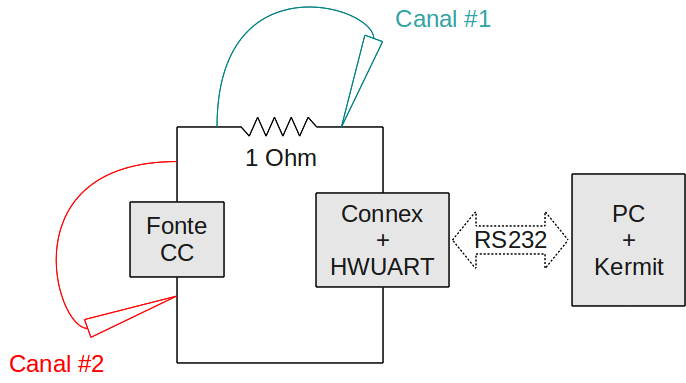
\includegraphics[scale=0.5]{fig/setup.png}
  \end{center}
  \caption{Evaluation setup}
  \label{fig:experiment}
\end{figure}


Despite the quick and flexible development, the GNU Radio data flow model imposes some limitations for implementing simultaneous radio chains. Both paths share the same USRP2 block, thus they must be on the same flow graph. But the GNU Radio model requires both paths to be running at the same time, and stopping one of the radio chains blocks the entire flow graph. We were able to overcome this by implementing a demux using stall blocks. These stall blocks can simply pass the inputs directly to the outputs or they can consume all the inputs and generate no outputs, thus we can easily switch between 802.11b and 802.15.4 block chain without blocking the entire flow graph. The figure~\ref{fig:structure} shows the implemented structure in GNU Radio and the \textit{demux} details. 

\begin{figure}
  \begin{center}
    \includegraphics[scale=0.5]{fig/structure.png}
  \end{center}
  \caption{Structure implemented in GNU Radio and Demux detail}
  \label{fig:structure}
\end{figure}



\section{Evaluation of the Proposed Approach}
\label{sec:results} 

To achieve the equipment flexibility proposed in Section~\ref{sec:sdr_wsn} is necessary the evaluation of critical parameters, such as the impact of latency caused by the physical layer reconfiguration. Table~\ref{tab:latencies} shows the results of four kinds of time latency for physical layers reconfiguration, which are described below:

\begin{itemize}
 \item[-] \textit{T\subscript{init}} is the time to create the flow graph and make all connections, which only occurs at start-up of system.
 \item[-] \textit{T\subscript{conf}} is the time to configure the USRP2 for the new physical layer, where are set a new center frequency and decimation rate, which are the hardware parameters that vary between 802.11b and 802.15.4
 \item[-] \textit{T\subscript{lock}} is the time to stop the flow graph responsible for implementing the physical layer.
 \item[-] \textit{T\subscript{unlock}} is the time to release the flow graph again.
\end{itemize}


\begin{table}[!h]
    \caption{Time of Initialization and Configuration}\begin{center}
        \begin{tabular}{|l|r|r|} \hline
                                   & \textbf{802.15.4}     & \textbf{802.11b}           \\ \hline
            T\subscript{init}      & \unit{98.72}\milli\second     & \unit{4.2}\milli\second        \\ \hline
            T\subscript{conf}      & \unit{1.04}\milli\second      & \unit{0.94}\milli\second        \\ \hline
            T\subscript{lock}      & \unit{12.9}\micro\second     & \unit{19.1}\micro\second        \\ \hline
            T\subscript{unlock}    & \unit{11.9}\micro\second     & \unit{25.1}\micro\second        \\ \hline
        \end{tabular}
        \label{tab:latencies}
    \end{center}
\end{table}


Thus the times to exchange between physical layers are given by the following formulas:

% \begin{eqnarray*}
%     T_{802.15.4\rightarrow802.11b} = & T_{lock\_802.15.4} & + \\
%                                      & T_{conf\_802.11b}  & +  \\
%                                      & T_{unlock\_802.11b}&
% \end{eqnarray*}
% 
% \begin{eqnarray*}
%     T_{802.11b\rightarrow802.15.4} = & T_{lock\_802.11b}   & + \\
%                                      & T_{conf\_802.15.4}  & +  \\
%                                      & T_{unlock\_802.15.4}&
% \end{eqnarray*}

\begin{eqnarray*}
    T_{PHY1\rightarrow PHY2} = & T_{lock\_PHY1} & + \\
                                     & T_{conf\_PHY2}  & +  \\
                                     & T_{unlock\_PHY2}&
\end{eqnarray*}



The final values of table~\ref{tab:exchange} were obtained as described above. The time to exchange between PHY layer 802.15.4 by the 802.11b is \unit{0.98}\milli\second~ and the inverse spends \unit{1.07}\milli\second. The really relevant latency is the \textit{T\subscript{conf}}, which makes sense, due the configuration of USRP2 hardware depends on the drivers and the communication channel, it should bear more interferences of intrinsic system latencies.

\begin{table}[h!]
    \caption{Time to exchange the Physical Layer}\begin{center}
        \begin{tabular}{|c|c|}    \hline
            \textbf{802.15.4 $\rightarrow$ 802.11}  & \textbf{802.11 $\rightarrow$ 802.15.4}    \\ \hline
            \unit{0.98}\milli\second      & \unit{1.07}\milli\second                            \\ \hline
        \end{tabular}
        \label{tab:exchange}
    \end{center}
\end{table}


Despite the exchange time is not being large and not impeding the SDR gateway, a SDR running in a dedicated system has many advantages in this context. Without the interferences of a generic processing environment, like a Personal Computer (PC) used by the GNU Radio, the exchange of PHY layer should be faster. In fact, there are better SDR platforms than GNU Radio and USRP2 for commercial embedded system applications, such as Bell Labs Programmable Radio Platform~\cite{ackland:2005} or Embedded SDR~\cite{Balister:2007}. However, even these embedded platforms consume more resources than simple nodes to give more connectivity and flexibility, thus the research to determine the gateway numbers and their locations in the network can be used to balance this trade-off~\cite{Youssef:2007}.

The magnitude of latency to exchange physical layers allows the creation of a multi-PHY architecture for providing services to upper layers. This flexibility can be used directly by application or by Data Link and Network layers to meet the communications requirements set by the user. Moreover, this architecture can be useful to provide vertical mobility within the various networks available in order to equalize the best data transfer rate, range and power savings.

%As the gateways consume more resources to give more connectivity and reliability, the research to determine the gateway numbers and their locations in the network can be used to balance this trade-off.~\cite{Youssef:2007} introduces an approach for estimating the least number of gateways required for meeting some upper bound on data latency and present a heuristic for finding the best locations for these gateways.



\section{Conclusions and Future Work}
\label{sec:conclusion}
In this paper, we suggest the use of SDR nodes to have more versatility in WSN gateways, which can assume different behaviors to increase flexibility and connectivity of WSNs. Three scenarios were shown and discussed, but there are other applications in WSN that can use the versatility of SDR.

Furthermore, we used a Software Defined Radio technology to present the analyses of time latency of dynamic exchange between 802.15.4 PHY and 802.11b PHY, which can be extrapolated for any other physical layers. Our experiment showed that even for a entire physical reconfiguration the magnitude of latency is not prohibitive.

As future work, we want to improve the PHY layer exchange structure to allow the integration with novels WSN architectures and upper layers. Another interesting field of research is the search of low-power SDR to employ in real WSN applications. Moreover the algorithms to determine connectivity problems and to coordinate the PHY layers modifications are great research challenges. 




\bibliographystyle{IEEEtran}
\bibliography{IEEEabrv,wsn_sdr}


\end{document}


